\begin{figure}[ht]
  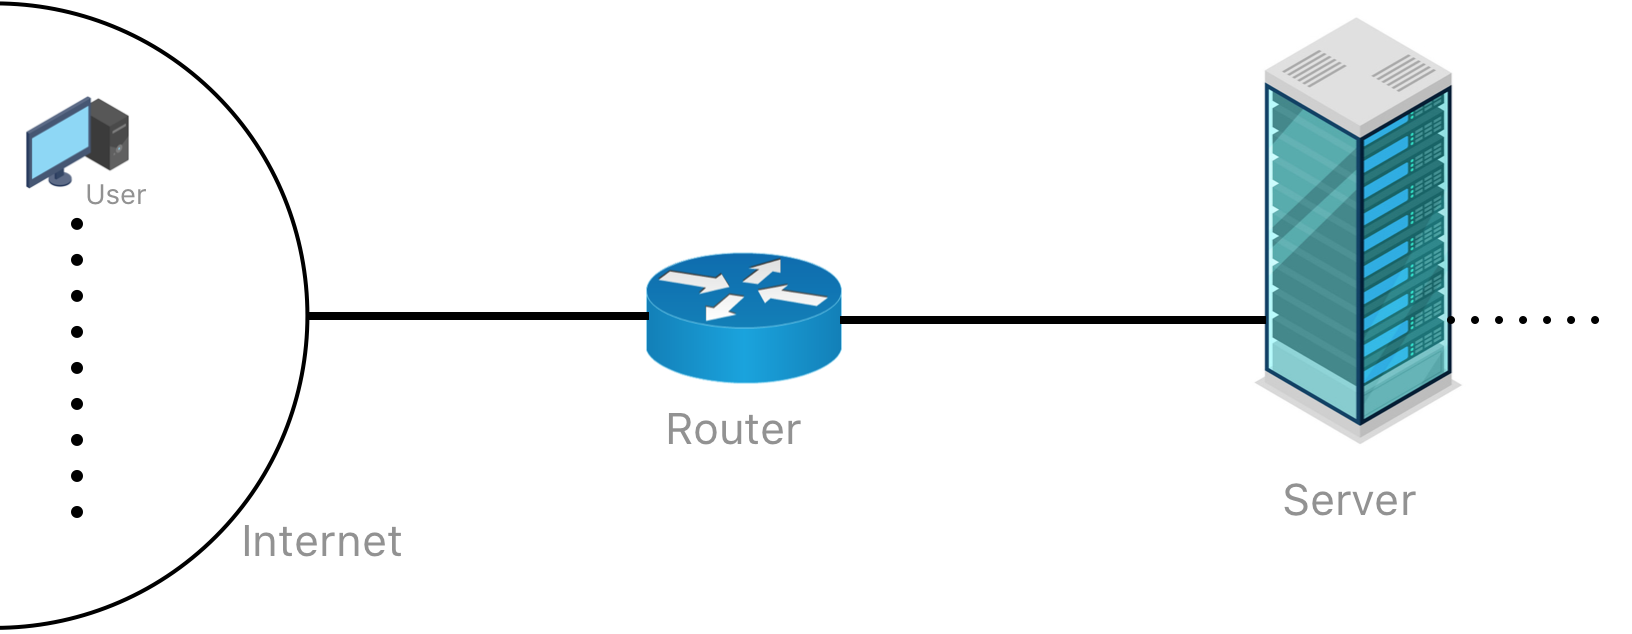
\includegraphics[scale=0.31]{imgs/scenario.png}
  \caption{Network Scenario}
  \label{fig:networkscenario}
\end{figure}

\begin{figure*}[h]
	\begin{subfigure}{0.48\textwidth}
		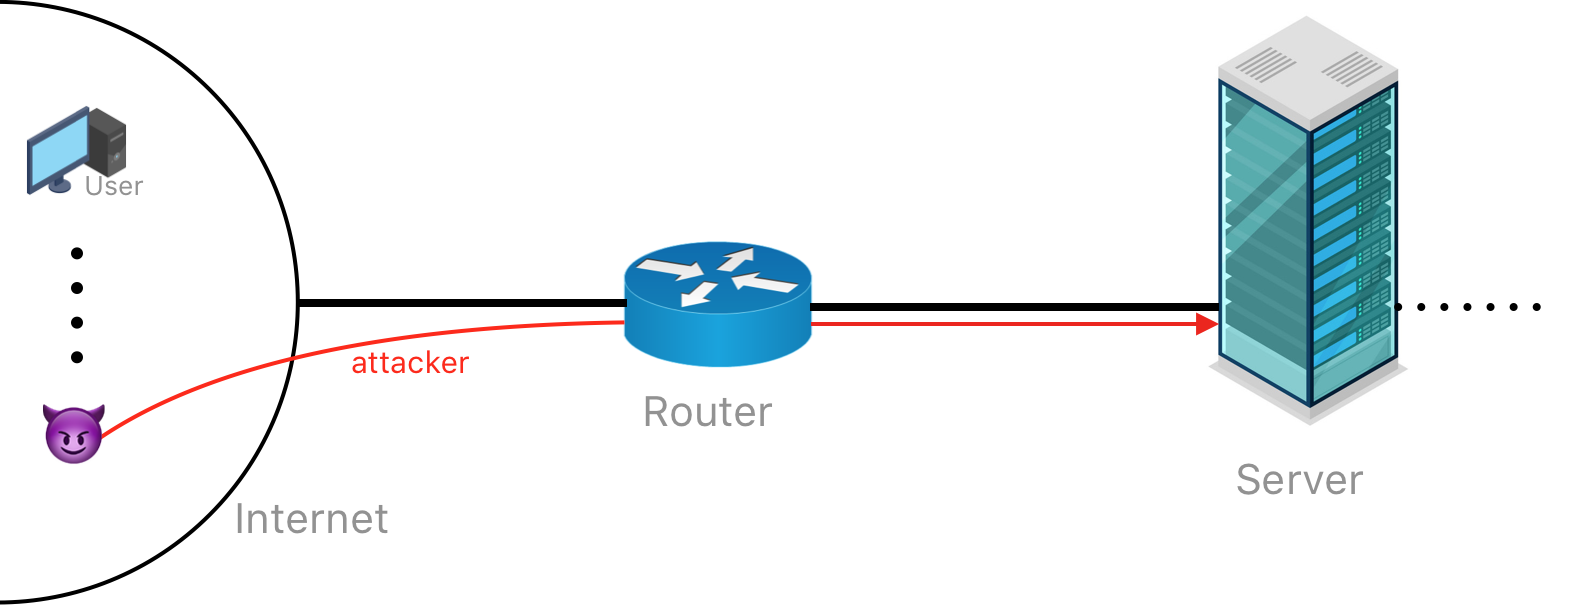
\includegraphics[width=\textwidth]{imgs/DoS_attack.png}
		\caption{DoS attack scenario} \label{fig:DoS}
	\end{subfigure}
	\hspace*{\fill} % separation between the subfigures
	\begin{subfigure}{0.48\textwidth}
		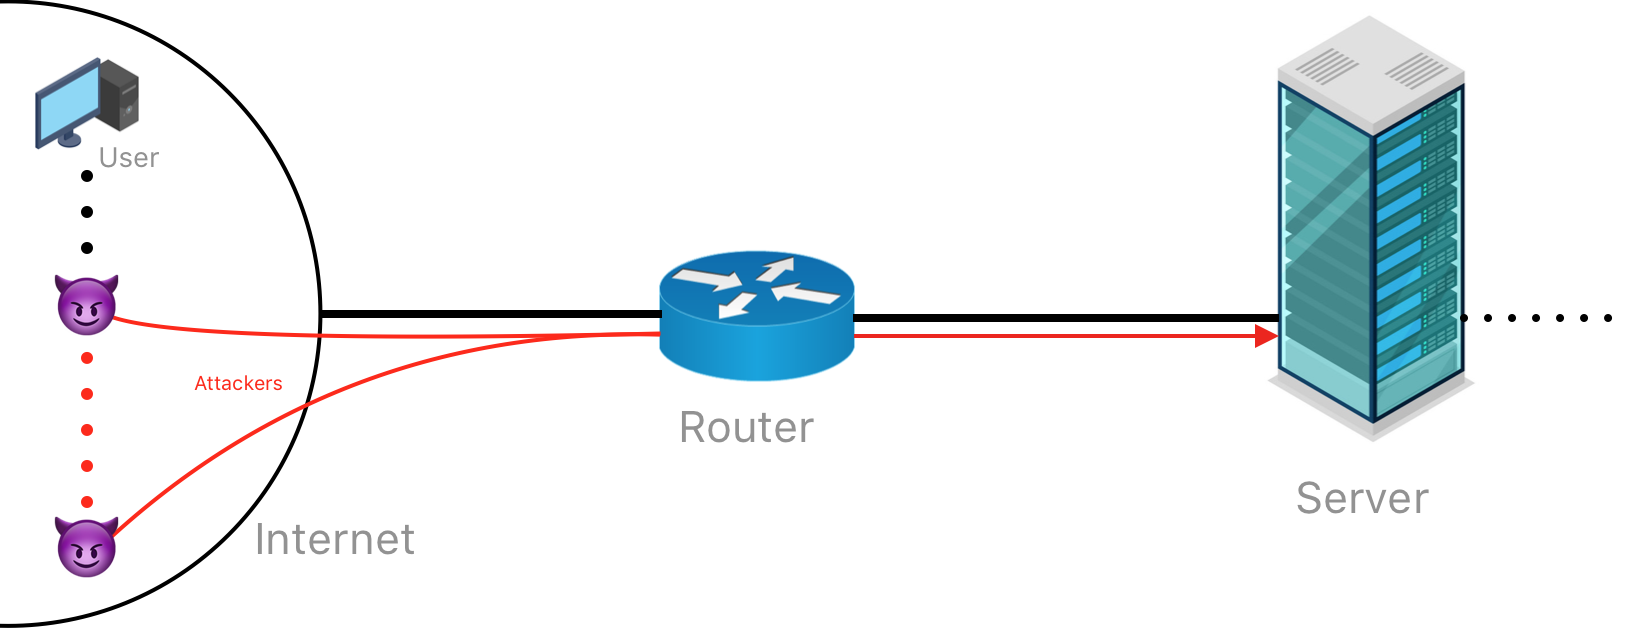
\includegraphics[width=\textwidth]{imgs/DDoS_attack.png}
		\caption{DDoS attack scanrio} \label{fig:DDoS}
	\end{subfigure}
	\caption{Attacks scenarios}
	\label{fig:atks}
\end{figure*}

\section{Analysis}
In this section we will illustrate the scenario on which we have tested our tool, traffic analysis is mainly based on IP addresses and timestamp\cite{ddos_forensics}.More over we will show two examples of attack, DDoS and DoS, in order to explain and evaluate our analysis quality trying to base our conclusion by using different datasets\footnote{Mentioned dataset were generated by our tool, it is possible to analyse every type of dataset on your own if in \texttt{pcap} format.}. There is also a summary of how to configure and run an analysis with \textit{Python} and \textit{Hadoop}.

\subsection{Configuring and Running Analysis}
This tool has been developed for running analysis over network flow records with minimal effort from the user. Once installed and configured \textit{Hadoop} on your PC or cluster, only one line of code is needed for running and storing the results of an analysis, as shown in the example below

\begin{lstlisting}[firstline=1, lastline=1]
   python3 DDoSAnalysis.py -a dataset_name
	Write('Case insensitive '); 
	WritE('Bash keywords.')
\end{lstlisting}

\subsection{Scenario} 
The scenario we focusing on is illustrated in fig.\ref{fig:networkscenario}, as we can see it is a very simple and basic design scenario. There is a \textit{router} that communicates with \textit{internet},  it connects the \textit{sever} with the global network, as we will see further on the treatment \textit{internet} may contains one or several attackers which aim is to deny the service give by the \textit{server}. 

In this scene common users exchange with the server at least 650 MB, the upper bound is $800$ MB with an average speed of $2.2$ Kb/s during the user server connection lifecycle. These data comes from an analysis in normal\footnote{Dataset generated without attackers in order to get an estimation of normal traffic conditions.} server condition, these assumptions are based on a \textit{log} file with a pool of one hundred users. As we will se further this assumption is the ground truth for our analysis under attacks condition.

We choose this type of network configuration in order to concentrate our heed on the implementation of analysis tools and big data scripting, which are the main topics of this project.
 


\subsection{DoS Analysis Example}

\subsection{DDoS Analysis Example}




















